\section{Reducción de dimensionalidad}

\subsection{Introducción}
Este ejercicio consistió en reducir la dimensión original de los datos, la cual era de 850, en un espacio de 9 componentes. El objetivo fue el de capturar
las componentes que mas explican la variabilidad de los datos en un espacio de dimensión menor. Para esto se utilizaron redes neuronales entrenadas con
los algoritmos de \textit{Oja} y \textit{Sanger}.

\subsection{Desarrollo}
La red neuronal que se utilizó para reducir dimensionalidad fué un perceptron simple con función de activación lineal. Esta red contó con 850 neuronas de entrada y
 9 neuronas de salida. Esta topología fue pensada para poder obtener una neurona de salida por cada clase posible de palabra y poder asi capturar la variabilidad de cada
 una.

Los algoritmo utilizados para el entrenamiento fueron los de \textit{Oja} y \textit{Sanger} cuyos pseudocodigos se presentan a continuacion:
%%%%%%%%%%%%%%%%%%%%%% PONER PSEUDO DE OJA Y SANGER %%%%%%%%%%%%%%%%%%%%%%%%%%%%%

Se decidió separar el conjunto de datos en entrenamiento y testing con una proporcion de 90\% y 10\% respectivamente. Los hiperparametros utilizados para el entrenamiento
de la red fueron $\eta = 0.0001$ y 500 epocas. La razon por la que se decidió utilizar un coeficiente de entrenamiento de una magnitud tan pequeña fue que los datos de entrada
no estaban normalizados, logrando que ocurran errores de overflow.

\subsection{Resultados}
Para una visualización mas clara de los datos se decidieron realizar tres graficos diferentes en el que cada uno muestra de a tres componentes principales. Se decidieron graficar los
datos de testing con un marcador con forma de triangulo para diferenciarlo de los circulos que representan los datos de entrenamiento. Los resultados
obtenidos se presentan a continuacion:


\begin{figure}[H]
  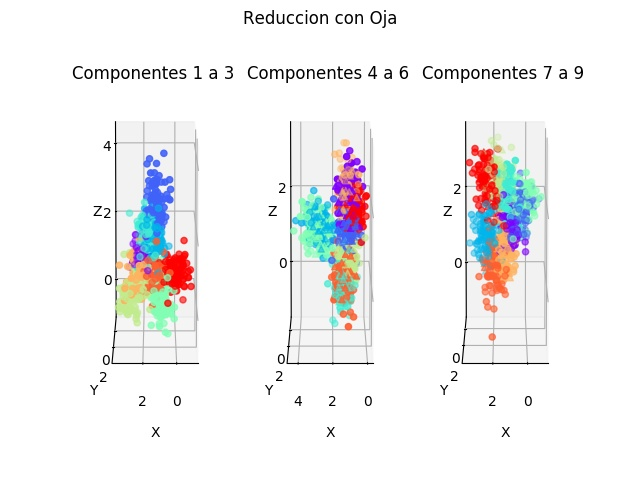
\includegraphics[width=125mm]{imagenes/reduccion_Oja_1.jpg}
  \caption{Vista desde arriba con Oja}
\end{figure}

\begin{figure}[H]
  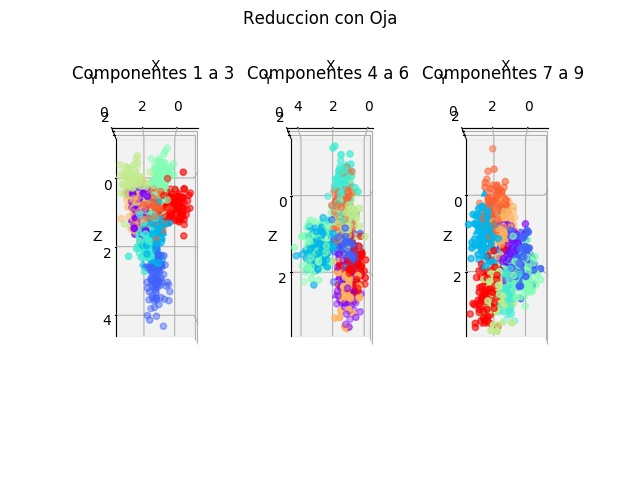
\includegraphics[width=125mm]{imagenes/reduccion_Oja_2.jpg}
  \caption{Vista desde abajo con Oja}
\end{figure}

\begin{figure}[H]
  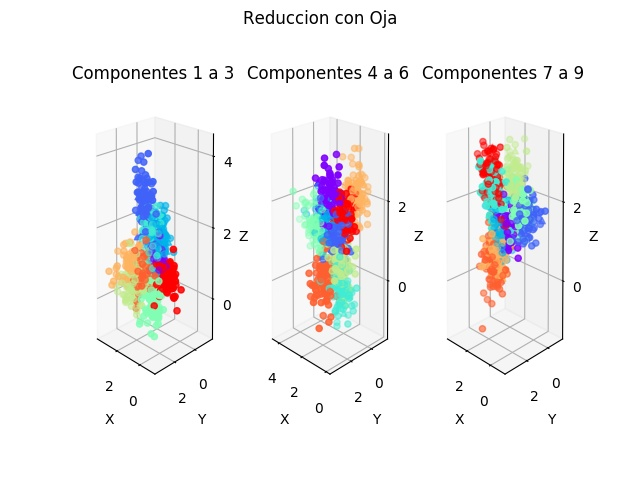
\includegraphics[width=125mm]{imagenes/reduccion_Oja_3.jpg}
  \caption{Vista de costado con Oja}
\end{figure}

\begin{figure}[H]
  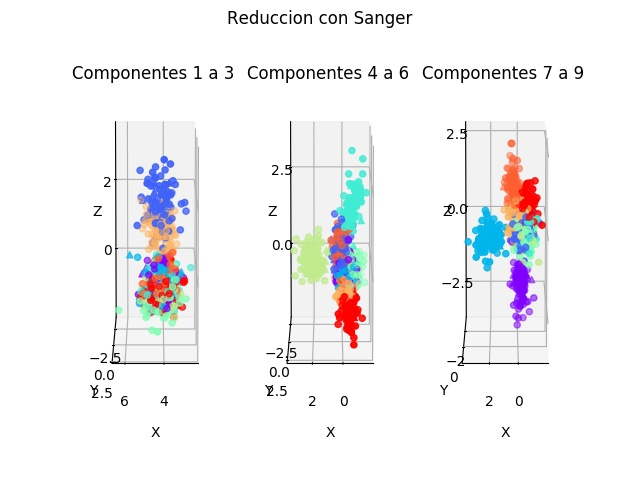
\includegraphics[width=125mm]{imagenes/reduccion_Sanger_1.jpg}
  \caption{Vista desde arriba con Sanger}
\end{figure}

\begin{figure}[H]
  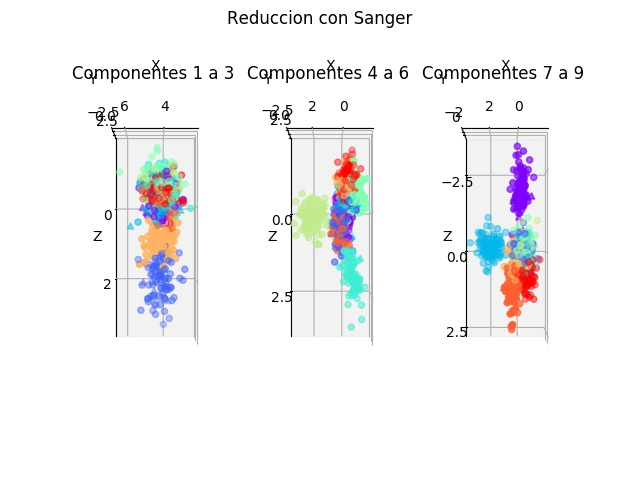
\includegraphics[width=125mm]{imagenes/reduccion_Sanger_2.jpg}
  \caption{Vista desde abajo con Sanger}
\end{figure}

\begin{figure}[H]
  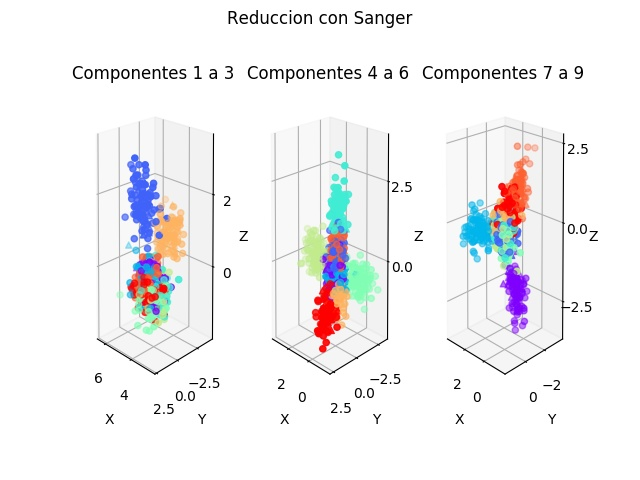
\includegraphics[width=125mm]{imagenes/reduccion_Sanger_3.jpg}
  \caption{Vista de costado con Sanger}
\end{figure}

\subsection{Conclusión}

\newpage
